\documentclass{beamer}
\usepackage{tcolorbox}
\usepackage{graphicx}
\usepackage{amsmath}
\usepackage[labelformat=empty]{caption}
\usepackage{subcaption}

\usepackage{hyperref}
\hypersetup{
    colorlinks=true,
    linkcolor=blue,
    filecolor=magenta,      
    urlcolor=cyan,
}

\usepackage{tikz}
\def\checkmark{\tikz\fill[scale=0.4](0,.35) -- (.25,0) -- (1,.7) -- (.25,.15) -- cycle;} 


%\beamerdefaultoverlayspecification{<+->}
\newcommand{\data}{\mathcal{D}}

\DeclareMathOperator*{\argmin}{arg\,min}
\DeclareMathOperator*{\argmax}{arg\,max}

\newcommand\Item[1][]{%
	\ifx\relax#1\relax  \item \else \item[#1] \fi
	\abovedisplayskip=0pt\abovedisplayshortskip=0pt~\vspace*{-\baselineskip}}
	


\usetheme{metropolis}           % Use metropolis theme


\title{Active Learning}
\date{\today}
\author{Nipun Batra}
\institute{IIT Gandhinagar}
\begin{document}
  \maketitle

\begin{frame}{The need for Active Learning}
\vspace{1cm}
Supervised Learning:
\begin{itemize}
\item Uses a lot of data to train models
\item Labeled data is hard to \textbf{obtain} and \textbf{expensive} to make.
\end{itemize}
\pause
But, most of the time the data that we feed into the model do not have any effect on the model.
\begin{figure}
        \begin{subfigure}[b]{0.5\textwidth}
                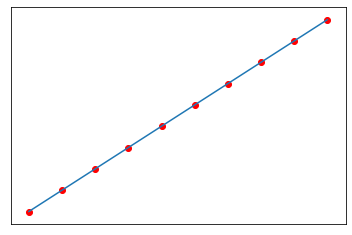
\includegraphics[width=\linewidth]{active/in_1.png}
        \end{subfigure}%
        \begin{subfigure}[b]{0.5\textwidth}
                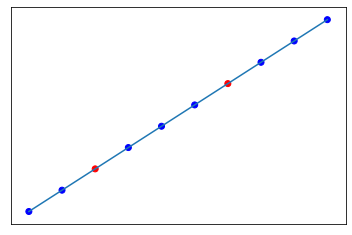
\includegraphics[width=\linewidth]{active/in_2.png}
        \end{subfigure}%
\end{figure}
\end{frame}

\begin{frame}{The need for Active Learning: Intuition}
Obtaining unlabeled data is relatively easier. \\So using it we can:
\begin{itemize}
\item<2-> identify those points that add the most information
\item<3-> label them
\item<4-> use this data to train the model
\end{itemize}
\end{frame}

\begin{frame}{Sampling Scenarios}
Different techniques by which the most important data points are identified. They include:
\begin{itemize}
\item\alt<2>{Membership Query Analysis: learner generates an instance (based on an underlying distribution) that is sent to an oracle to be labeled.}{Membership Query Analysis}
\item\alt<3>{Stream Based Sampling: The learner chooses weather to query or reject a generated data instance based on its informativeness}{Stream Based Sampling}
\item\alt<4>{Pool Based Sampling: The learner analyzes the an entire \emph{pool} of unlabeled data is analyzed, ranked and then queried for the best data points}{Pool Based Sampling}
\end{itemize}

\end{frame}

\section{Query Strategies}

\begin{frame}{Uncertainty Sampling}
\vspace{0.6cm}
\textbf{Basic Idea:} Find the point that you are most uncertain about.
\vspace{-0.6cm}
\begin{figure}
\begin{overprint}
\onslide<2> 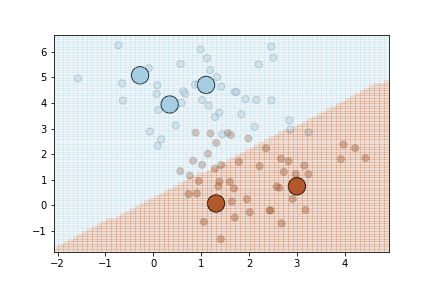
\includegraphics[width=\textwidth]{active/un_1.png}
\onslide<3> 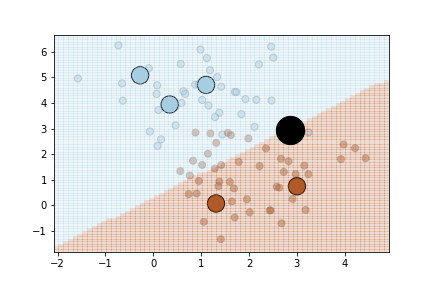
\includegraphics[width=\textwidth]{active/un_2.png}
\onslide<4-> 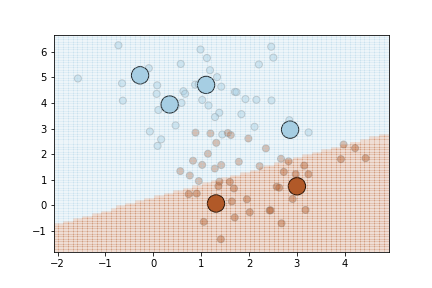
\includegraphics[width=\textwidth]{active/un_3.png}
\end{overprint}
\end{figure}
\end{frame}

\begin{frame}{Uncertainty Sampling: Finding the data point}

Least Confidence Estimate: 
$$
x_{LC}^* = \argmax_{x} \left(1 - P_\theta\left(\hat{y}\left(x\right)\right)\right)
$$
Where, $\hat{y}$ is the class with the max probability
\pause
\bigskip \\
Margin Sampling:
$$
x_{m}^* = \argmin_{x}  \left(P_\theta\left(\hat{y_1}\left(x\right)\right) - P_\theta\left(\hat{y_2}\left(x\right)\right)\right)
$$
Where, $\hat{y_1}$ and $\hat{y_2}$ are the classes with the max probability
\end{frame}

\begin{frame}{Query by Committee}
In query by committee, we maintain a committee $C = \left\lbrace \theta^1, theta^2, \ldots , theta^C \right\rbrace$ that are trained on the same labeled set ($L$) but represent \emph{competing} hypothesis.
\pause \\ \bigskip
Each committee member (model) votes and the point that sees the most amount of disagreement is considered to be the most informative instance. 
\end{frame}

\begin{frame}{Query by Committee}
Example: For a QBC with Random Forest, we have 
\begin{align*}
\theta^1 &= \text{ Model 1 = R.F. with seed 1} \\
\theta^2 &= \text{ Model 2 = R.F. with seed 2} \\
\ldots
\end{align*}
\pause
\\ \bigskip
For the case of regression, we can compute the variance amongst the committee and chose that data point that has the most variance as the most informative one.
\end{frame}

\begin{frame}{Extra Reading and References}
\href{https://sammed98.github.io/Distil_Pub_Article/}{Active Learning; Ayush Garg and Sammed Kagi} \\ \bigskip
\href{https://colab.research.google.com/drive/1HMPn0mpMAe4XFe5Zvh4oExgi5evkgjTi}{Google Colab Link}
\end{frame}

\end{document}